\chapter{Konzeption}
\label{chap:konzept}
    In diesem Kapitel wird das erarbeitete Konzept dieser Arbeit dargelegt. Basierend auf den 
    Anforderungen, die aus den Anwendungsfällen, den Experteninterviews und der Zielgruppenanalyse 
    erhoben wurden, werden die daraus generierten Überlegungen und Entscheidungen transparent 
    dargestellt. Durch die bereits erfolgten Schritte der Anforderungsanalyse (siehe Kapitel \ref{chap:anforderungsanalyse})
    sind erste Schritte der Konzeption abgeschlossen. 
    \\
    Zu Anfang des Kapitels wird das allgemeine Ziel eines Konzeptes, sowie das konkrete Ziel dieser Arbeit 
    erläutert. Anschließend 
    wird auf das Anwendungsumfeld des Systems, bzw. des Frameworks, (\ref{sec:anwendungsumfeld}) eingegangen, darunter 
    welche zusätzlichen Komponenten notwendig sind, damit das Framework in einer dafür vorgesehenen Umgebung sinnvoll 
    eingesetzt werden kann.
    % die abzudeckenden Funktionalitäten (\ref{sec:konzeptfunktionalitaet}), die 
    %aus den Anforderungen ermittelt wurden, eingegangen. 
    Darauf folgend wird anhand den 
    zugrundeliegenden Informationen und Anforderungen das Architekturkonzept (\ref{sec:architekturkonzept}) erläutert. %, sowie das 
    %Softwarekonzept (\ref{subsec:softwarekonzept}) erläutert. 
    Dabei wird auf verschiedene kontextabhängige Aspekte, sowie Sichtweisen der Anwender und des Frameworks eingegangen.
    Die Darstellung des Konzeptes stützt sich mit Diagrammen und Veranschaulichungen.
    %Des Weiteren werden die Hintergründe der 

\section{Ziel der Konzeption}
\label{sec:konzeptziele}
    Das Ziel einer Konzeption ist die Veranschaulichung von abstrakten Ideen, geistiger Entwürfe und Leitideen. 
    Hierbei werden aus den zugrundeliegenden Problemstellungen, Szenarien und Anforderungen Entwürfe und 
    Lösungsmöglichkeiten erarbeitet und identifiziert. Diese helfen bei der Aufstellung von notwendigen Schritten 
    und dienen als Grundlage zur Untermauerung und Darlegung von Entscheidungen. Somit wird Dritten der Kontext, die 
    Domäne und das zu lösende Problem, bzw. die Lösung dargestellt. 
    \\
    \linebreak
    Im Rahmen dieser Arbeit ist das Ziel des Konzeptes die Veranschaulichung der Entscheidungsfindung zur Lösung des vorliegenden 
    Sachverhaltes. Das Konzept 
    erarbeitet eine Lösung zur Implementierung einer Anwendung, die es ermöglicht, Automatisierungen, Regeln und Prozesse innerhalb eines 
    Firmenbüros zu koordinieren. Der Fokus liegt dabei verstärkt auf der einfachen Nutzung des Frameworks für den Anwender und 
    die uneingeschränkte Ausprägungsvielfalt von Regelprozessen. Dadurch kann der Anwender die vorgegebene Struktur nutzen, um individuelle 
    Sachverhalte zu realisieren, die in seinem Umfeld abzudecken sind. 
    %\\
    Hierfür wird der allgemeine Aufbau der Architektur skizziert und demonstriert, wie eine solche Lösung aussehen kann. 
    Unter Berücksichtigung der Forschungsfrage (siehe Abschnitt \ref{sec:forschungsfragen}) wird eine Möglichkeit offengelegt, mit der 
    ein Softwareentwickler neue Regeln entwickeln und dem System hinzufügen kann, ohne ein weiteres zu erlernendes Framework zu verwenden. 
    Dabei sollen die notwendigen Schritte und Interaktionen formalisiert und für den Entwickler vereinfacht werden. Mit der 
    Definition der Zielsetzung der Arbeit (siehe Abschnitt\ref{sec:zielsetzung}) wird die Abgrenzung deutlich. 
    \\
    \linebreak
    In folgender Darlegung %des Konzeptes 
    wird nochmals konkreter auf den Kontext als auch auf die Intension der Arbeit eingegangen. 
    % Das Ziel des Konzeptes ist es, dem Entwickler den Aufwand zur Erweiterung des Systems zu minimieren durch weitere 
    % Regeln und Abdeckung von Anwendungsfällen (Use Cases) und eine Struktur vorgeben. (ToDo's, Flexibilität in der 
    % Umsetzung (nicht wie Home Assistant und openHAB eher eingeschränkt)) 

%\section{Abzudeckende Funktionalitäten}
%\label{sec:konzeptfunktionalitaet}
    % Was soll der Entwickler machen können? 
    % Welche Grundlagen braucht er, um eine Regel implementieren zu können?
    % Welche Funktionen müssen gegeben sein, um die Struktur vorzugeben? 
    % Reicht ein Hinweis weöche Stellen angepackt werden müssen, um eine Regel hinzuzufügen? 
    
    %%%%%%%%%%%%%%%%%%%%%%%%%%%%%%%%%%%%%%%%%%%%%%%%%%%%%%%%%%%%%

    % ZIEL DES KONZEPTES: Ein Framework für Entwickler bereitzustellen, welches die Mächtigkeit für den Entwickler offen lässt, nicht einschränkt 
    % und dennoch Konfiguration und Ausführung umsetzt. Der Entwickler muss lediglich den Zustandsraum, die MQTT-Topics und die Regeln definieren.
    % Der Entwickler bekommt ein Framework an die Hand, welches die Umsetzung von Prozessen in einem smarten Büro ermöglicht. Das Framework kümmert sich um die 
    % Organisation und die Ausführung der Regeln. Die Richtigkeit der Regeln und des Zustandsraumes muss der Entwickler sicherstellen. 
    % Die Kommunikation über MQTT ist nur eine Möglichkeit. Das Setup wird wegabstrahiert 

    %%%%%%%%%%%%%%%%%%%%%%%%%%%%%%%%%%%%%%%%%%%%%%%%%%%%%%%%%%%%%

\section{Anwendungsumfeld}
\label{sec:anwendungsumfeld}
    Grundsätzlich ist der Einsatzort des Frameworks variabel, da die eigentliche Implementierung und Nutzung der Regeln und Prozesse stark 
    abhängig von den Anwendern ist. Dadurch kann sowohl im privaten \acl{SH} Umfeld als auch in Büroräumen ein System mittels dem 
    Framework erstellt werden. Basierend auf den vorangestellten Tätigkeiten, darunter die Anforderungsanalyse und die Eingrenzung auf den 
    Einsatz im Smart Office, liegt der Schwerpunkt der Arbeit auf dem Einsatz in einem smarten Büro. 
    \\
    \linebreak
    Stützend auf den vorab ermittelten Anwendungsfällen (siehe Abschnitt \ref{subsec:checkin} und \ref{subsec:evacuation}) sind unabhängige 
    Komponenten, darunter bspw. ein Service-Roboter und weitere einsatzfähige Geräte, sowie ein \acs{MQTT}-Broker notwendig. Ein \acs{MQTT}-Broker 
    wird im Zuge der Konzeption nicht von dem Framework bereitgestellt, lediglich die Anbindung als Client wird gegeben, und muss daher als eigenständige 
    Instanz bereitgestellt werden. Dadurch kann die Anforderung, die Kommunikation mittels \acs{MQTT}, ermöglicht werden. Eine mögliche infrastrukturelle 
    Architektur kann wie folgt aussehen: 
    \begin{figure}[hbt!]
        \centering
        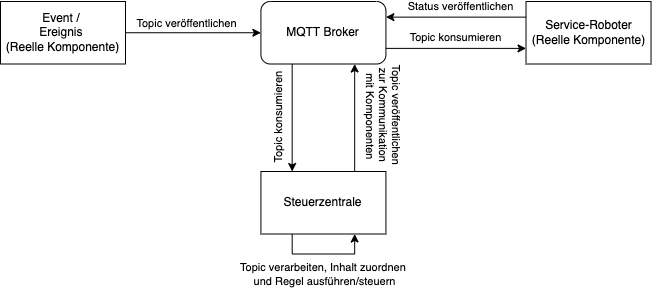
\includegraphics[width=14cm,height=11cm,keepaspectratio]{images/Systemarchitektur.png}
        \caption{Infrastruktur des Anwendungsumfeldes der Steuerzentrale}
        \label{fig:infrastructure}
    \end{figure}

\section{Konzept}
\label{sec:concept}
    Die Intension, die hinter der Ausarbeitung dieses Konzeptes steht, ist zum einen die einfache Handhabung der 
    formalisierten Interaktionen für Softwareentwickler %während
    unter der Verwendung des Frameworks und zum anderen die 
    offene Gestaltung von Regelprozessen. Dadurch ist der Anwender bei der Implementierung von Regeln, Aufgaben und Automatisierungen 
    für ein intelligentes Büro nicht eingeschränkt und kann mit der Regeldefinition flexibel variieren.
    %einzugrenzen zu beschränken. 
    Es soll lediglich ein Muster vorgegeben werden, damit Regeln einheitlich als solche von dem Framework 
    verarbeitet und genutzt werden können. 
    \\ 
    \linebreak
    In vergleichbaren Softwareprodukten, die im Rahmen dieser Arbeit erläutert 
    wurden (siehe Kapitel \ref{sec:homeassistant} und \ref{sec:openhab}), ist die Vielfalt der Regelausprägung auf 
    den Kontext des Systems eingeschränkt. Dies bedeutet, dass 
    Regeln und Prozesse nur mit Komponenten und Informationen innerhalb des Systems arbeiten können, bzw. benötigte 
    Informationen erst durch eine systemseitige Erweiterung durch Plugins verfügbar sind, auf die der Nutzer keinen direkten 
    Einfluss nehmen kann. Diese Auswirkung ist unter anderem der 
    Tatsache geschuldet, dass mit den bestehenden Lösungen versucht wird, die Regeldefinition für Endnutzer so 
    einfach wie möglich zu gestalten. 
    \\
    %\linebreak
    Um dennoch dem Anwender eine Struktur vorzugeben, mit der Regeln definiert und zur Laufzeit der Anwendung ausgeführt 
    werden können, soll mit diesem Konzept ein Framework erarbeitet werden, dass diese Herausforderungen löst. Hierfür soll 
    dem Anwender die Komplexität der Regelverwaltung und deren Durchführung nicht vorgehalten werden. Dieser ist lediglich 
    in der Verantwortung, die für ihn notwendigen Regeln und Prozesse zu definieren und dem Framework bereitzustellen. 
    Dadurch soll der Person, die das Framework verwendet, die Möglichkeit geboten werden, das zur Verfügung gestellte System 
    mit individuellen Regeln, dafür vorgesehene Bedingungen, Komponenten und dessen Zustände zu implementieren. Beispielsweise 
    können bei Regeldefinitionen Informationen direkt von Datenpunkten über \acs{HTTP} Abfragen bezogen werden, bzw. Ressourcen 
    und Inhalte individuell nachgezogen werden.
    \\ 
    Das Konzept beinhaltet die in folgendem Abschnitt dargelegten Komponenten. Aus denen bildet sich der grundlegende Aufbau 
    des Frameworks.

    \subsection{Konzeptkomponenten}
    \label{subsec:conceptcomps}
        Für die Erläuterung des Konzeptes werden vorab die einzelnen Konzeptkomponenten erläutert, da diese die Anhaltspunkte 
        für den weiteren Verlauf darstellen: % . Das Framework baut auf folgenden Bausteinen auf:
        \begin{itemize} 
            \item Regel (Rule): Eine Regel ist ein Konstrukt, welches bei bestimmten Events die darin enthaltenen Aktionen ausführen soll. 
            Der grobe Aufbau einer Regel ist immer gleich. Diese beinhaltet einen Auslöser, eine Bedingung, einen Prozess und einen eindeutigen 
            Namen. Die Inhalte der Regel kann der Anwender ja nach bedarf beliebig ausprägen und ergänzen. 
            \item Komponente (Component): Eine Komponente soll einen reellen Gegenstand abbilden, der bei Benutzung durch eine Regel unter anderem 
            für weitere Regeln gesperrt und freigegeben werden kann. 
            \item Zustandsraum (State): Der Zustandsraum, das sog. Zustandsobjekt, soll alle Zustände von Komponenten und weiteren Geräten abbilden. 
            \item Auslöser (Trigger): Ein Auslöser löst im Allgemeinen eine bestimmte Aktion aus. Im Kontext des Frameworks gibt es zwei Ausprägungen von 
            Auslösern. Zum einen werden eingehende Aktionen entgegengenommen und über die Transformation verarbeitet, zum anderen können durch Regelprozesse 
            Aktionen und weitere Schritte ausgelöst werden. Dadurch werden ausgehende Aktionen gesteuert. 
            %Der Auslöser ist unter anderem ein von außen einwirkendes Objekt, das Zustandsänderungen hervorruft. Beispielsweise ist ein 
            %Auslöser das eintreffen eines Events über eine Kommunikationsschnittstelle. Ebenso können durch Regelprozesse Events ausgelöst werden. 
            \item Transformation (Transformer): Mit der Transformation werden eingehenden Zustandsänderungen, die durch ein Event ausgelöst werden, 
            auf das eigentliche Zustandsobjekt übertragen. 
            %, die eine Zustandsänderung bewirken, die durch einen Auslöser hervorgerufen 
            %werden und eine Zustandsänderung bewirken
        \end{itemize}
        Diese Komponenten bilden den Kern des Frameworks.
        %In folgendem Abschnitt wird nochmals auf die Sichten eingegangen und anhand denen der Ablauf des Frameworks als auch die 
        %Aufgaben des Anwenders erläutert. %Der Ablauf des Prozesses von Auslöser bis zur Ausführung der Regel wird anhand eines Programmablaufdiagramms gestützt.
        \\
        %\linebreak
        Das Konzept wird aus zweierlei Sichtweisen betrachtet, die in folgendem Abschnitt aufgegriffen werden und für die weitere 
        Konzepterläuterung notwendig sind.
    
    \subsection{Sichtweisen}
    \label{subsec:sichtweisen}
        Wie bereits aus dem Kontext hervorgeht, wird das Konzept auf zwei Sichtweisen aufgeteilt. Zum einen auf die 
        Anwendersicht, die der Softwareentwickler als entscheidende Kraft einnimmt, indem dieser das Aufsetzen und in 
        Betrieb nehmen des Systems, sowie das Definieren und Implementieren von Regeln übernimmt. Zum anderen die 
        Bereitstellungssicht, die das Framework als ausführende Kraft besetzt. Dieses sorgt für die Ausführung der vom 
        Anwender definierten Regeln. Ebenso stellt es Funktionen bereit, die das Empfangen von Events und das starten 
        von Regeln ermöglicht. Das Management zum Starten von Regeln und Prozessen wird in Gänze vom Framework übernommen. 
        Das Konzept widmet sich grundlegend dem initialen Aufbau des Frameworks. Zum besseren Verwalten und Starten von 
        Prozessen können weitere Konzepte und Managementroutinen ergänzt werden. Diese sind nicht Teil dieses Konzeptes und 
        werden im Ausblick zu möglichen Erweiterungsschritten nochmals aufgegriffen.
        \\
        \linebreak
        Zusammenfassend wird zwischen den beiden Sichtweisen differenziert, da diese Trennung ein elementarer Schnitt des Konzeptes 
        aufzeigt. Die Sichten werden konkretisiert, indem die Aufgaben des Anwenders als auch der Ablauf innerhalb des Frameworks 
        erläutert wird.
        % dafür, dass für das Setup benötigte Funktionen bereitstehen und vom Anwender definierte Regeln 
        %ausgeführt werden. 
        \\
        \linebreak
        Der Anwender hat das initiale Setup des Frameworks zur Aufgabe. Zuerst sollte der Zustandsraum erstellt werden. 
        Darin sind alle notwendigen Zustände als Attribute abzubilden. Diese können konkret Geräte sein, die im Rahmen des 
        intelligenten Büros verwendet werden können, bspw. ein Service-Roboter, ein Türöffner und weitere steuerbare Geräte, die 
        ihren Zustand ändern können. Nachdem das Zustandsobjekt 
        definiert wurde, geht es an die Definition und Implementierung der Regeln. Diese sind individuell, je nach 
        Anforderungen des Anwenders zu erstellen. Jedoch sind bestimmte Funktionen und Vorgaben bezüglich Bedingungsprüfung 
        und Prozessdurchlauf einzuhalten. Anforderungen dabei sind das Implementieren von drei unabdingbaren Funktionen. 
        Die erste Funktion ist die Zuordnung des Auslösers, damit klar wird, durch welches Event eine Regel ausgelöst werden kann. 
        Die zweite zu implementierende Funktion ist die Prüfung von Werten im Zustandsraum, sodass beim eintreffen spezifischer 
        Bedingungen und Zuständen bestimmte Regelprozesse ausgeführt werden können und die dritte vorgegebene Funktion ist die 
        des tatsächlichen Regeldurchlaufes. Die darin enthaltenen Aufgaben werden nach eintreffender Anforderungen, durch Prüfung der 
        vorangestellten Bedingungen, abgearbeitet.
        %Zum einen die Prüfung einer Bedingung, die zutreffen muss, damit ein bestimmter Prozess ausgelöst wird
        %, die zum einen die 
        %Bedingungen gegen Werte im Zustandsobjekt zu prüfen und zum anderen das Nutzen der Prozessfunktion, damit der Inhalt 
        %der Regel durchlaufen wird.
        \\
        Nach Fertigstellung aller Regeln, müssen diese in einer Liste an das System übergeben werden. Anschließend sind die 
        Kommunikationswege zu aktivieren. 
        Da \acs{MQTT} zum aktuellen Zeitpunkt und zur Abdeckung der Anforderungen die einzige Kommunikationsschnittstelle 
        abbildet, ist die Konfiguration des \acs{MQTT} Clients einzustellen. Hierfür muss der Entwickler 
        dem Framework den Host des \acs{MQTT}-Brokers, sowie den Nutzername des Clients und dessen Passwort übergeben. Über das 
        Framework wird dann das Setup durchgeführt, sodass Topics (Themen), die über den Broker veröffentlicht werden, konsumiert 
        werden können. In Zuge dessen muss der Anwender alle Topics definieren und dem Framework übergeben. Dadurch wird gewährleistet, dass 
        die Steuerzentrale nur auf die Topics hört, die der Anwender bekannt gegeben hat. Abschließend muss der Softwareentwickler 
        noch die Zuordnung der Topics implementieren. Hierbei muss fest vorgegeben werden, mit welcher \acs{MQTT} Nachricht ein 
        bestimmter Wert, bzw. ein bestimmtes Attribut im Zustandsraum geändert werden soll. Hierfür ein Beispiel: 
        \\
        Sobald eine Person an der Tür authentifiziert wurde, wird ein Thema mit dem Namen derjenigen Person übergeben. Basierend auf 
        dem eingehenden Topic wird dann für dieses Ereignis der Wert im Zustandsraum auf den Namen der Person geändert. Somit kann 
        die Steuerzentrale mit dem neuen Wert und der Änderung des Zustandsraumes arbeiten. Durch die Zustandsänderung wird dann 
        geprüft, ob eine Regel für diese bestimmte Änderung definiert wurde. Trifft diese Bedingung zu, so wird der dazugehörige Regelprozess 
        durchlaufen.  
        \\
        %\linebreak
        Sind diese Schritte abgearbeitet, so sind die Pflichten des Anwenders erfüllt und die Steuerzentrale kann gestartet werden. 
        %\\
        Hierfür wird der Durchlauf von dem Eingang einer \acs{MQTT} Nachricht bis zur Ausführung einer Regel aus Sicht des Frameworks 
        erläutert.
        \\
        \linebreak
        Nach erfolgreichem Einstellen und Starten des Systems soll der \acs{MQTT} Client hochgefahren werden. Dieser baut darauf hin eine 
        Verbindung zu dem \acs{MQTT} Broker auf und startet das Zuhören auf eingehende Themen. Dabei soll bereits auf die Topics,  
        die der Nutzer über die Einstellungen als Liste aller Topic-Zeichenketten übergibt, gefiltert werden. Sobald eine der bekannten 
        \acs{MQTT} Nachrichten konsumiert wird, soll mittels des Transformers der Zustandsraum, bzw. das Zustandsobjekt 
        auf die in dem Topic enthaltenen Informationen abgeändert werden. Der Transformer stellt den Ausgangspunkt für die Transformation 
        des Inhaltes der Nachricht zur Änderung des Zustandsobjektes dar. Innerhalb dieser Komponente findet die Zuordnung 
        des Topics zu den darauf adressierten Instanzvariablen des Zustandsobjektes statt. Mittels der Nachricht sollen die Informationen dieser 
        in den Attributwert der durch den Entwickler spezifizierten Variable übertragen, bzw. überschrieben werden. Die Änderung des 
        Zustandsraumes löst darauf hin den weiteren Ablauf aus. 
        \\
        Das aktuelle Zustandsobjekt wird zum Zeitpunkt der Überschreibung für Lese- und Schreiboperationen gesperrt, sodass 
        die Gültigkeit des Zustandsraumes nicht erlischt. Anschließend erfolgt die Erstellung einer Kopie des Zustandsobjektes, mit der 
        darauf folgend weiter verfahren wird. Für die Zeitspanne der Zustandsänderung und der 
        nachfolgenden Kopie soll das Zustandsobjekt kurzzeitig für weitere Transaktionen und Änderungen, genauer gesagt für Lese- und 
        Schreiboperationen durch einen Lock-Mechanismus gesperrt werden. Dadurch kann anschließend das Zustandsobjekt mit der vorher 
        getätigten Änderung kopiert werden, um die anschließende Regel-Iteration durchzuführen. Wichtig an dieser Stelle zu 
        erwähnen ist, dass die Prüfung der Regel-Bedingungen mit der Kopie durchgeführt werden soll.
        Durch den Sperrvorgang wird gewährleistet, dass eine Zustandsänderung sauber durchgeführt wird und darauf hin eine Regel mit der 
        Kopie des Zustandsobjektes ausgelöst werden kann. Hierdurch ist sichergestellt, dass jeweils eine Zustandsänderung zu einem 
        Zeitpunkt stattfindet und zu dieser die dafür definierte Regel ausgeführt wird, sofern die Bedingung im Vorfeld ebenso zutrifft. 
        %\\
        Wird kurz darauf eine weitere Nachricht konsumiert, so kann das aktuelle Zustandsobjekt dahingehend überschrieben und erneut 
        kopiert werden. Die Kopie wird wiederum für die Regel-Iteration verwendet und tangiert die vorherige Kopie nicht. Somit soll 
        zu jedem Zeitpunkt der aktuelle Zustandsraum repräsentiert werden. Davon ausgehend entspricht dieser immer der Wahrheit.
        \\
        \linebreak
        Dem folgenden Diagramm ist der abstrakte Programmablauf des Frameworks, welcher soeben skizziert wurde, zu entnehmen:
        \begin{figure}[hbt!]
            \centering
            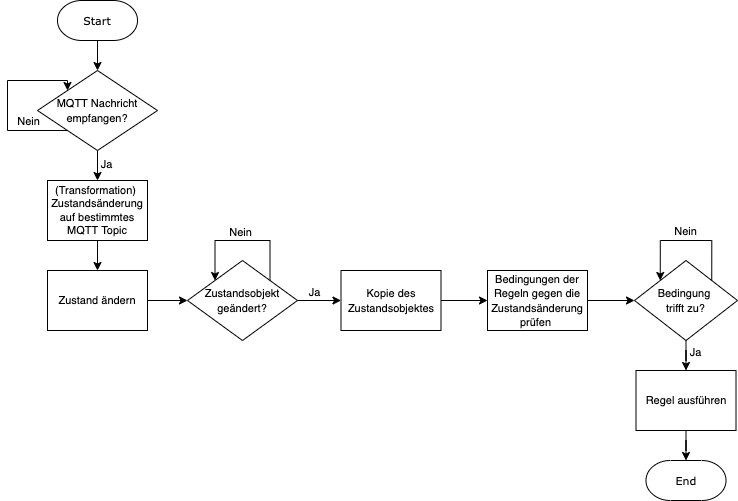
\includegraphics[width=14cm,height=11cm,keepaspectratio]{images/Programmablauf_Framework.png}
            \caption{Grober Programmablauf des Frameworks}
            \label{fig:programmablauf_framework}
        \end{figure}
        \\
        Aspekte, die nicht aus dem Ablaufdiagramm hervorgehen, sind zum einen die parallele Ausführung von zwei voneinander unabhängigen 
        Zustandsänderungen und zum anderen die erneute Änderung des Zustandes durch eine Regel selbst. Sofern die Änderungen unabhängig 
        sind, sollen Prozesse auch asynchron ablaufen, bzw. Regeln auch neue Zustandsänderungen hervorrufen können. Die genauere Ausprägung des 
        Konzeptes wird im Rahmen des Architekturkonzeptes (\ref{sec:architekturkonzept}), sowie dem Kapitel der Umsetzung 
        (\ref{chap:umsetzung}) aufgegriffen. 
        %\\
        %\linebreak
        Zur Veranschaulichung der abgeschlossenen textuellen Erläuterung des Konzeptes hilft die nachfolgenden Abbildung: 
        